\chapter{Concluding chapter}
\label{ch:conclusion}

\begin{enumerate}
\item We used observational data to understand how longer and warmer seasons change growth for juvenile and mature trees
	\begin{enumerate}
	\item Our findings are significant as they show that forest recruitment may not be harmed by climate change
	
	\item Mature trees store most of the forests carbon and we found that adult trees may not grow more with future warmer seasons 
	
	\item Only one species out of 11 decreased growth with warmer seasons, so they may not grow more, but most don't seem to be harmed by warmer seasons
  
  \item However, this absence of trend could be due to a multi-year lag effect of carbon sequestration
  
  \item These findings reveal how the complex nature of climate change, coupled with the complex dynamic of tree growth, multiplied by large species differences, even when closely related makes these responses very complex to tease apart.
  
  \item This is why experiments would be useful to tease apart these climate drivers
  
	\end{enumerate}

\item Growing season extension and stressor experiments to complement thesis findings (Figure \ref{fig:effects})
  \begin{enumerate}
  \item In parralel to these two studies, I conducted an large-scale experiment during my MSc
  
  \item To disentengle the effect of longer seasons, we artifically submitted trees to spring and fall warming, in a full factorial design across seven species
  
  \item While I completed this experiment is completed and the data is collected, the data cleaning, analyses and writing will be part of my first PhD chapter, which I will start in January 2027.
  
  \item Alongside this experiment, I contributed to another experiment looking at the effect of the timing of spring frosts, droughts, also on juvenile trees and eight species.
  \end{enumerate}
  
\end{enumerate}


\begin{figure}[h!]
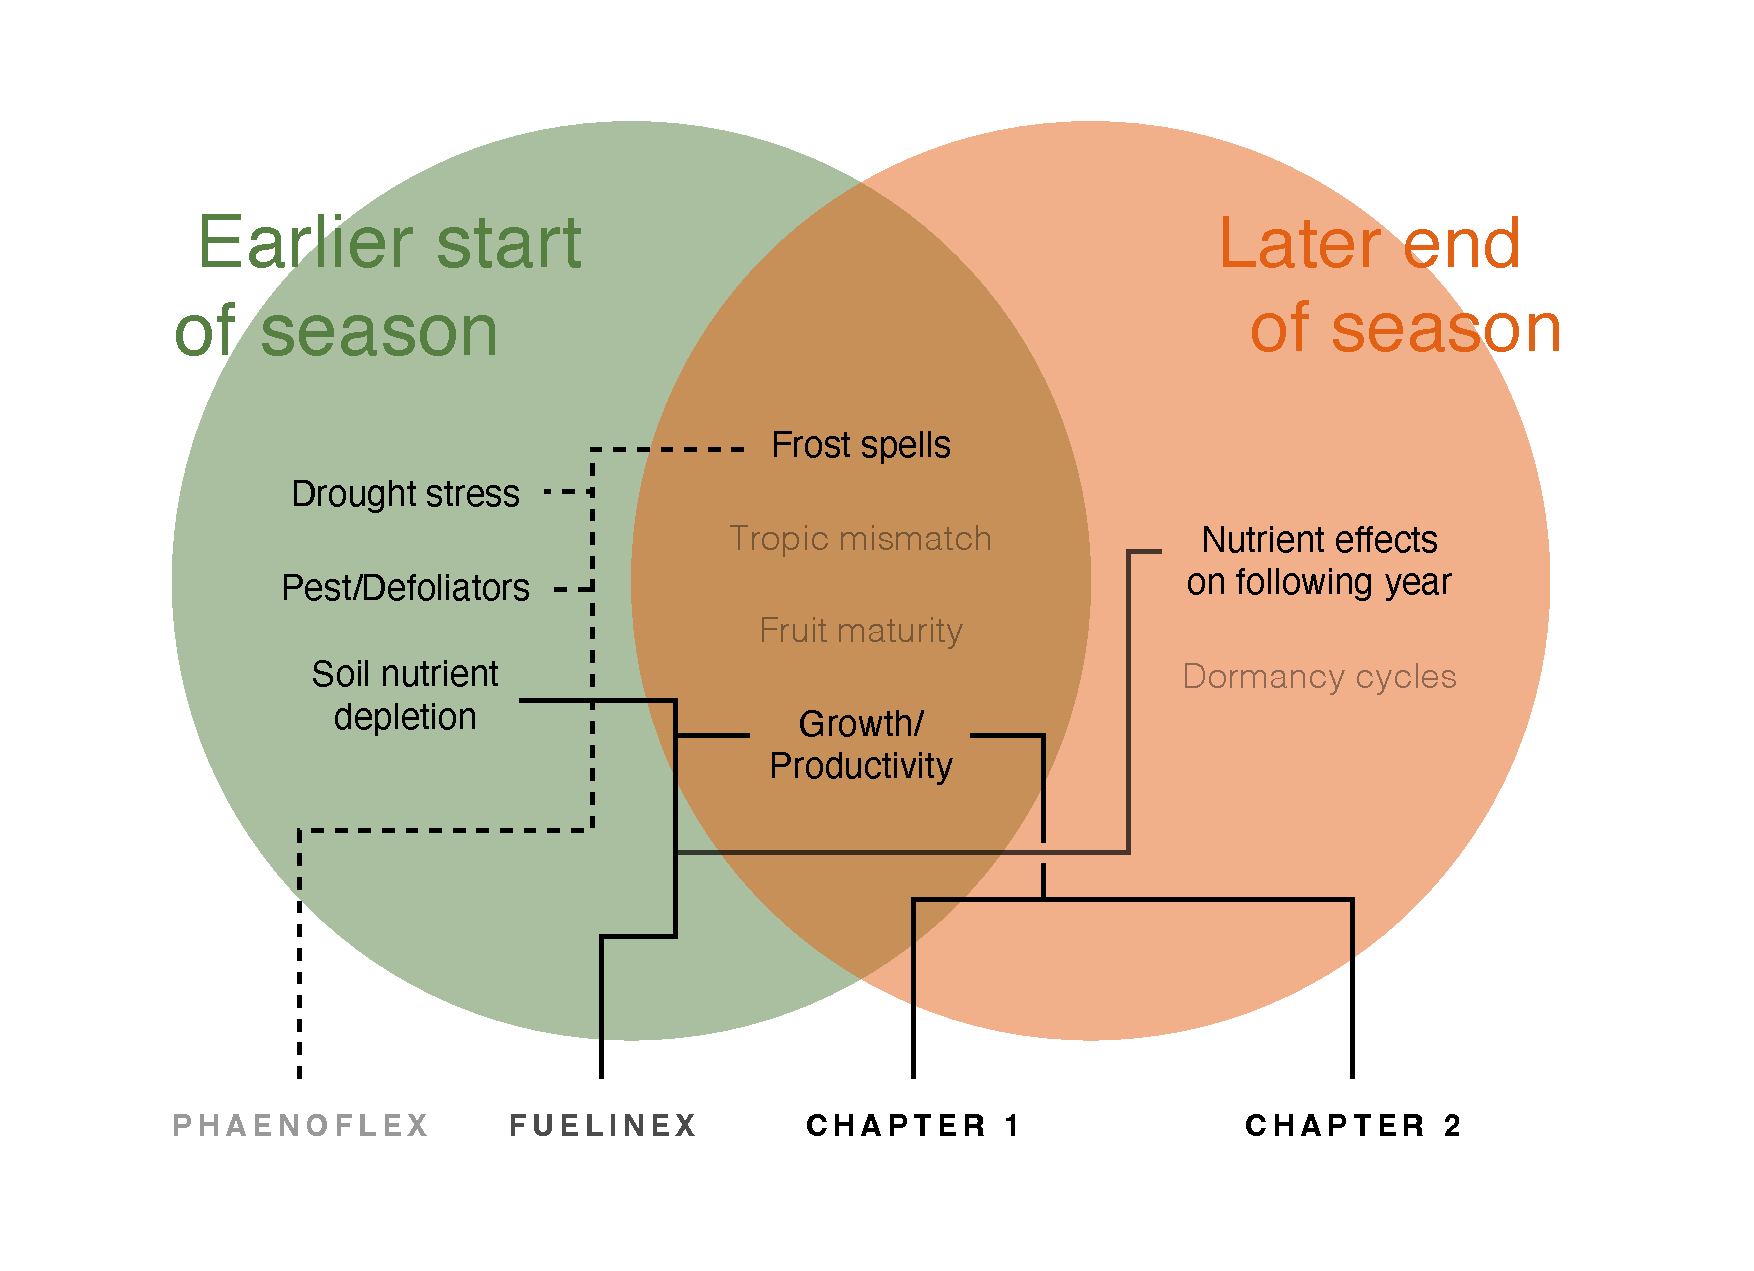
\includegraphics[width=0.8\textwidth]{../figures/studiedEffectsGSL.pdf}
\caption{The effects that an earlier start and later end of season can have on trees. Fuelinex is the experiment that I conducted over the course of my thesis and that will become my first PhD chapter. Solid lines connect the effects that I studied over the course of this thesis. Phaenoflex (in grey) and its dashed lines represent other effects I investigated in a related experimental project that I collaborated on in 2023 and 2024. }
\label{fig:effects}
\end{figure}